\documentclass[letterpaper,14pt,oneside]{report}
\usepackage{amssymb,amsmath,alltt}
\usepackage{graphicx}
\usepackage[latin1]{inputenc}
\usepackage[spanish]{babel}
\usepackage{setspace}
\usepackage{epsfig}
\usepackage{float}
\usepackage[10pt]{moresize}
\usepackage{titlesec}

%este es el archivo de configuracion
\usepackage{fancyhdr}
\usepackage[includeheadfoot,footskip=.5cm]{geometry}
\usepackage[small,bf]{caption}
%\usepackage{mathtools}
\usepackage{multirow}
\usepackage{array}
\usepackage{color, colortbl}
%
\pagestyle{fancy}
\geometry{lmargin=2cm,rmargin=3cm,tmargin=0.5cm,bmargin=4cm}
\def\arraystretch{1.5}

% Coloca una línea en los encabezados
\fancyhf{}
\fancyhead[L]{}
\fancyhead[R]{}
\fancyhead[C]{
	\begin{table}[H]
		\centering
		\begin{tabular}{ p{4.5cm} c p{1.6cm} }
		\multirow{3}{*}{
			
\includegraphics[width=0.25\textwidth]{images/logoecci.png}}
		 & ESCUELA COLOMBIANA DE CARRERAS INDUSTRIALES & \\
		 & GERENCIA DE PROYECTOS &\\
		 & &\hfill {\footnotesize GESPRO07}\\
		\end{tabular}
	\end{table}
}
% para mostrar el paginado
\fancyfoot[R]{\thepage}
\renewcommand{\headrulewidth}{0cm}
% Cambia la estructura de una página en blanco
\fancypagestyle{plain}{
\fancyhead[L]{}
\fancyhead[R]{}
\fancyhead[C]{
	\begin{table}[H]
		\centering
		\begin{tabular}{ p{4.5cm} c p{1.6cm} }
		\multirow{3}{*}{
			
\includegraphics[width=0.25\textwidth]{images/logoecci.png}}
		 & ESCUELA COLOMBIANA DE CARRERAS INDUSTRIALES & \\
		 & GERENCIA DE PROYECTOS &\\
		 & &\hfill {\footnotesize GESPRO07}\\
		\end{tabular}
	\end{table}
}
\renewcommand{\headrulewidth}{0pt}
}

% Cambia el ancho del encabezado
%\setlength{\headwidth}{16.5cm}

% Cambia el espacio para el encabezado
\setlength{\voffset}{5pt}
\setlength{\headheight}{70pt}
\setlength{\headsep}{0.5cm}

% Cambia el margen de los pies de figura
\setlength{\captionmargin}{10pt}

% Borra la palabra Capítulo del \chaptermark:
\renewcommand{\chaptermark}[1]{\markboth{\MakeUppercase
{\thechapter. #1}}{}}
% Quita la palabra capitulo
\addto\captionsspanish{\renewcommand{\chaptername}{}}

%definicion de colores
\definecolor{LightGrey}{gray}{0.9}
\definecolor{lgray}{gray}{0.75}
\definecolor{Grey}{gray}{0.7}

% Definiendo tamanos de los titulos
\titleformat{\chapter}
	{\bfseries\normalfont\normalfont}
	{\thechapter.}
	{6pt}
	{}
\titlespacing*{\chapter}{0pt}{0pt}{0pt}

\titleformat{\section}[block]
	{\Large\normalfont}
	{\thesection.}
	{6pt}
	{}
\titlespacing*{\section}{0pt}{0pt}{0pt}

\titleformat{\subsection}
{\normalfont\large\bfseries}{\thesubsection}{12pt}{}
\titleformat{\subsubsection}
{\normalfont\normalsize\bfseries}{\thesubsubsection}{12pt}{}
\titleformat{\paragraph}[runin]
{\normalfont\normalsize\bfseries}{\theparagraph}{12pt}{}
\titleformat{\subparagraph}[runin]
{\normalfont\normalsize\bfseries}{\thesubparagraph}{12pt}{}

%definiendo el modo de insercion de capitulos
\titleclass{\chapter}{top}

%definicion de recuadros gris y texto negro para secciones y capitulos
\titleformat{\chapter}[hang]{\Large\normalfont}{%
}{0em}{%
    {%
        \setlength{\fboxsep}{0pt}%
        \colorbox{lgray}{\makebox[\textwidth]{\Large\strut}}%
    }%
    \hspace*{-\textwidth}%
        {\thechapter}%
        \hspace*{1em}%
}[]
%
%\titleformat{\section}[hang]{\Large\normalfont}{6pt}{%
%    {%
%        \setlength{\fboxsep}{0pt}%
%        \colorbox{lgray}{\makebox[\textwidth]{\Large\strut}}%
%    }%
%    \hspace*{-\textwidth}%
%        {\thesection}%
%        \hspace*{1em}%
%}[]

% Se puede cambiar los siguientes parámetros para modificar el acomodo del texto
\parskip= 6pt
%definicion de los archivos

\begin{document}
\pagenumbering{arabic} \setcounter{page}{1}
\pagestyle{fancy}
\begingroup
\let\clearpage\relax
{\let\clearpage\relax\par%
\begin{table}[H]
	\centering
	\begin{tabular}{| c | c | c | c | p{1.5cm} | p{3cm} | }
	\hline
	\rowcolor{Grey}
	\multicolumn{6}{c}{CONTROL DE VERSIONES} \\
	\cline{1-6}\noalign{\smallskip}
	\hline
	\rowcolor{LightGrey}
	Versi\'on & Hecha por & Revisada por & Aprobada por & Fecha & Motivo \\ \hline
	1.0 & Javier Serrano & Yeymi Gonz\'alez & Jenny Fierro & Febrero 22 de 2015 & Creaci\'on de formato \\
	\hline
	2.0 & Javier Serrano & Yeymi Gonz\'alez & Jenny Fierro & Abril 10 de 2015 & Correciones para \newline segunda entrega \\
	\hline
	
	\end{tabular}
\end{table}
%}
{\let\clearpage\relax\par\chapter{OBJETIVO DE LA GESTI\'ON}

Integrar todas las \'areas del plan del conocimiento en un solo plan de Gesti\'on de Integraci\'on, 
y as\'i garantizar que se tengan en cuenta todas las actividades necesarias para lograr el objetivo 
del proyecto con \'exito.

\chapter{OBJETIVO DEL PLAN DE GESTI\'ON}

Documentar los procesos y la metodolog\'ia a utilizar para la implementaci\'on del proyecto.%}
{\let\clearpage\relax\par\chapter{PROCESOS A DESARROLLAR}
%
\section{Gesti\'on de m\'etricas}
Se desarrolla la gesti\'on necesaria para la recolecci\'on, definici\'on y trazabilidad
de los requerimientos pertinentes al proyecto.
%
\section{Scope statement}
Se recopila todos los requerimientos, se integra todo el proyecto y de requerimientos de producto.
%
\section{WBS}
Representaci\'on jer\'arquica del trabajo a ser realizado dentro del proyecto para: 
\begin{enumerate}
	\item alcanzar los objetivos del proyecto, y
	\item elaborar los entregables del proyecto (hardware, software, servicios y documentaci\'on).
\end{enumerate}
%
Presenta como caracter\'isticas principales:
\begin{itemize}
	\item Incluye todo el trabajo a realizar.
	\item Estructura jer\'arquicamente los distintos componentes del proyecto.
\end{itemize}
%
\section{Diccionario WBS}
Permite detallar cada \'item del WBS.}
{\let\clearpage\relax\par\chapter{REPORTES, DOCUMENTOS Y FORMATOS}
%
\section{Proceso: Gesti\'on de requerimientos}
%
\begin{itemize}
	\item \textbf{Reporte / Documentos}: Plan de gesti\'on de los requerimientos.
	\item \textbf{Formato}: requerimientos.pdf (GESPRO08)
\end{itemize}
%
%
\section{Proceso: Desarrollo del Scope Statement}
%
\begin{itemize}
	\item \textbf{Reporte / Documentos}: Scope Statement.
	\item \textbf{Formato}: scopestatement.pdf (GESPRO11)
\end{itemize}
%
\section{Proceso: Diagramaci\'on WBS}
%
\begin{itemize}
	\item \textbf{Reporte / Documentos}: WBS.
	\item \textbf{Formato}: wbs.pdf (GESPRO12)
\end{itemize}
%
\section{Proceso: Desarrollo del diccionario WBS}
%
\begin{itemize}
	\item \textbf{Reporte / Documentos}: Diccionario WBS.
	\item \textbf{Formato}: diccionariowbs.pdf (GESPRO13)
\end{itemize}}
{\let\clearpage\relax\par\chapter{T\'ECNICAS Y HERRAMIENTAS}
%
\begin{table}[H]
	\centering
	\begin{tabular}{| m{5cm} | c | p{5cm} |}
	\hline
	\textbf{PROCESO} & \textbf{T\'ECNICAS / HERRAMIENTAS} & \textbf{DESCRIPCI\'ON} \\ \hline
	5.1. Desarrollo del plan de gesti\'on & Lluvia de ideas & Definici\'on del grupo de actividades y herramientas 
	necesarias para la fase de integraci\'on del proyecto.\\
	\hline
	5.2. Desarrollo del Scope Statement & Alcance del proyecto & Con el Alcance se pueden definir cada uno de los 
	requerimientos y las funcionalidades que se quieren.\\ 
	  \cline{2-3}
	 & Juicio de expertos & Se identifica los Requerimientos con sus caracter\'isticas, prioridad y restricciones 
	 de los entregables. \\
	\hline
	5.3. Desarrollo diagrama WBS & Juicio de expertos & Con el consentimiento  de cada uno de los expertos en el 
	desarrollo del proyecto  se podr\'a finalizar exitosamente.\\
	\cline{2-3}
	& Alcance del proyecto & Tener en cuenta  los  requerimientos que el cliente quiere.\\
	\hline
	5.4. Desarrollo diccionario WBS & Documento de stakeholders & Se tiene en cuenta los interesados en el proyecto 
	y la funci\'on que cumple cada uno.\\
	\cline{2-3}
	& WBS & Tener la estructura de las fases y sus actividades.\\
	\cline{2-3}
	& Project charter & Se define la descripci\'on de cada integrante.\\
	\cline{2-3}
	& Juicio de expertos & Con esta t\'ecnica permitir\'a desarrollar quien intervendr\'a en cada una de las 
	actividades.\\
	\hline
	\end{tabular}
	
\end{table}}
{\let\clearpage\relax\par\chapter{PROCEDMIENTO}
%
\section{Desarrollo plan de gesti\'on de los stakeholders}
%
\begin{figure}[H]
    \centering
    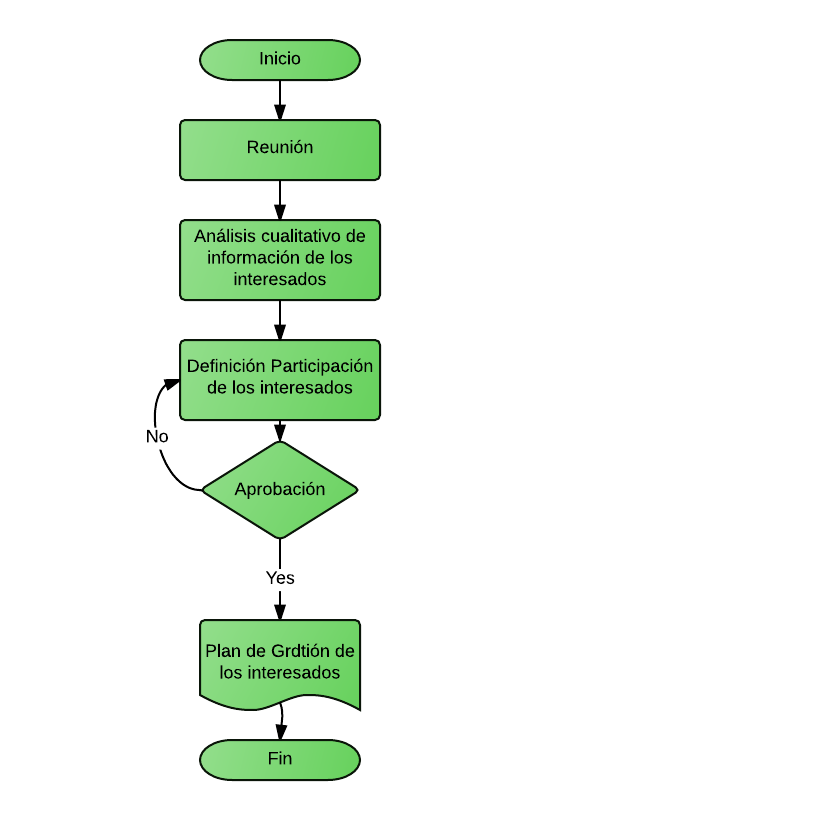
\includegraphics[width=1\textwidth]{images/gestion.png}
\end{figure}
%
\section{Registro de stakeholders}
%
\begin{figure}[H]
    \centering
    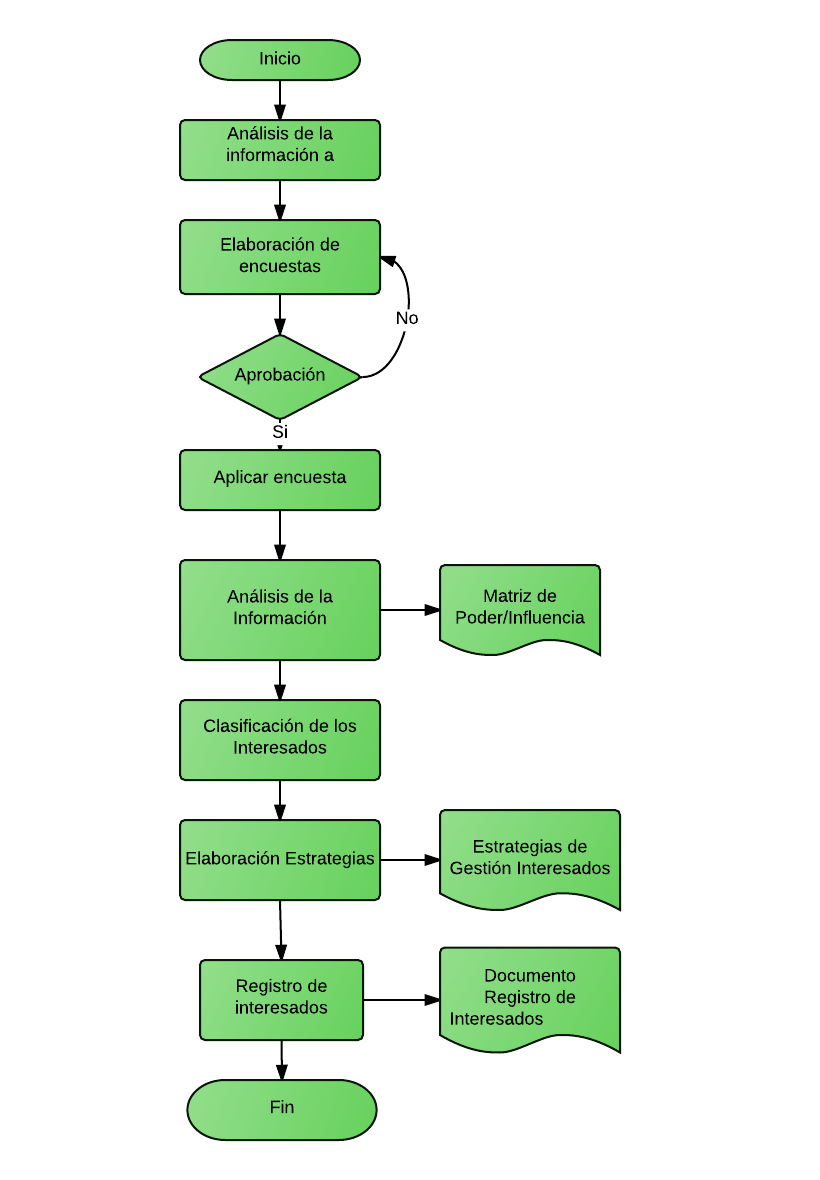
\includegraphics[width=0.8\textwidth]{images/registro.png}
\end{figure}}
\endgroup
\end{document}
